In the following paragraphs, tests on the accuracy for different
combinations of step sizes $\Delta x$ and $\Delta t$ are done. The
solution given by the three integration schemes are then compared
at two strategically chosen time points $t_1$ and $t_2$ so that at
$u(x, t_1)$ the solution is curved but smooth and at $u(x, t_2)$
the solution is approximately linear, close to the stationairy
state.

The test is done for $\Delta x = 1/10$ and $\Delta x = 1/100$.
$\Delta t$ is chosen to be the upper limit decided by the criterium
of stability \[ \alpha = \frac{\Delta t}{\Delta x^2} \leq
\frac{1}{2}. \] For the Crank Nicolson and Backward Euler scheme,
stability will not be decided by this criterium, yet equal grounds
for the simulation will make comparing more meaningful. This gives
the following test cases.

\begin{center}
\begin{tabular}[htbp]{|l|c|c|}
    \hline
    Case & $\Delta x$ & $\Delta t$ \\
    \hline
    \hline
    Case 1 & 1/10 = 0.1 & $1/200 = 5 \cdot 10^{-3}$ \\
    \hline
    Case 2 & 1/100 = 0.01 & $1/20000 = 5 \cdot 10^{-5}$ \\
    \hline
\end{tabular}
\end{center}

Through trial and error, strategic time points were chosen to be
the following.
\begin{align*}
    & t_1 = 0.085 & t_2 = 0.45
\end{align*}
Comparing the solution gave the plots shown in figure
\refig{case1} and \refig{case2}. The lines are overall close
together, yet the Forward Euler scheme seems to separate itself the
most from the other schemes. Because of the tight correlation,
differences are easier to make out on a different scale, as shown
in figure \refig{zoomed_schemes}.

\begin{figure}[htbp]
    \centering
    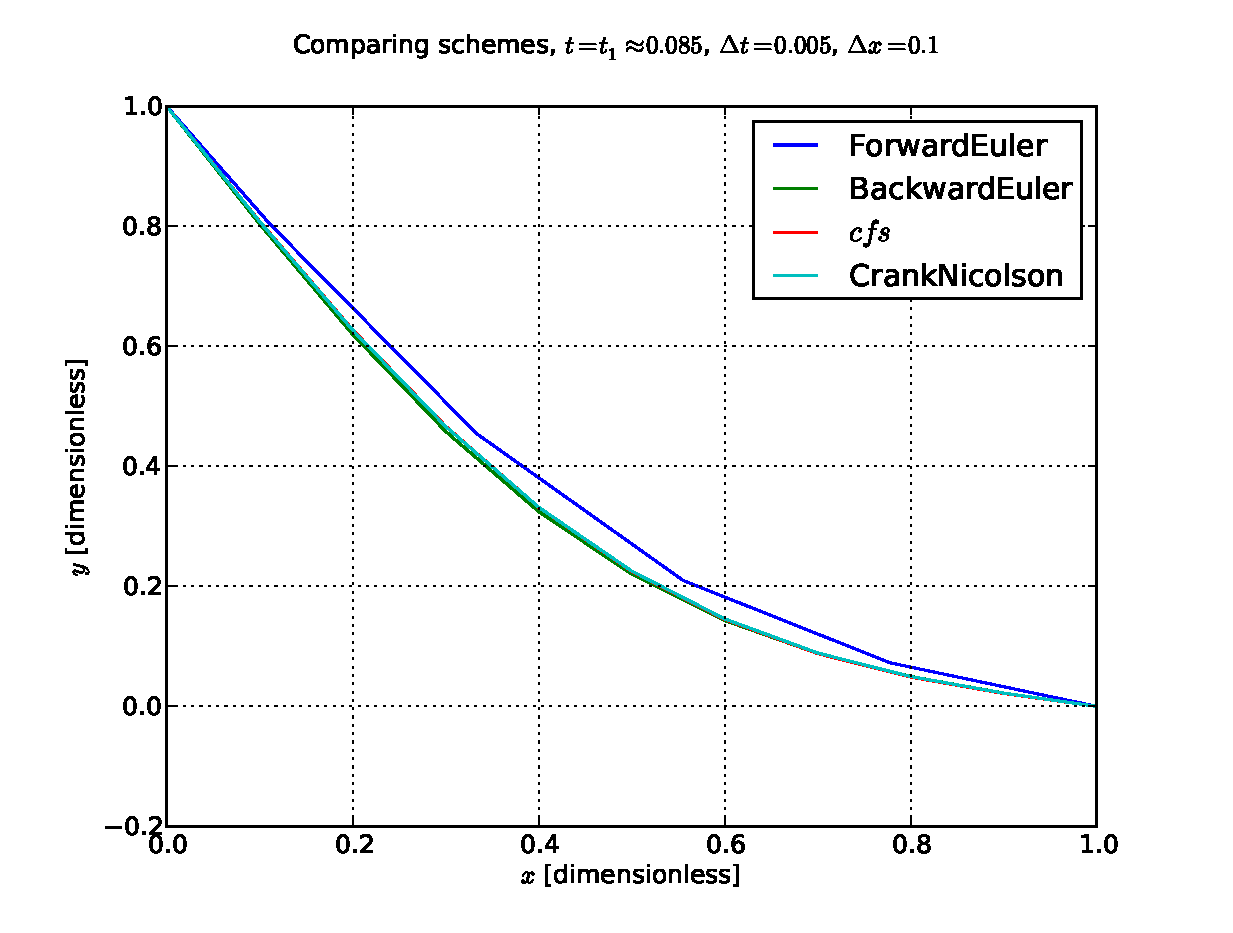
\includegraphics[width=0.9\textwidth]{plots/schemes_case1_t1.eps}
    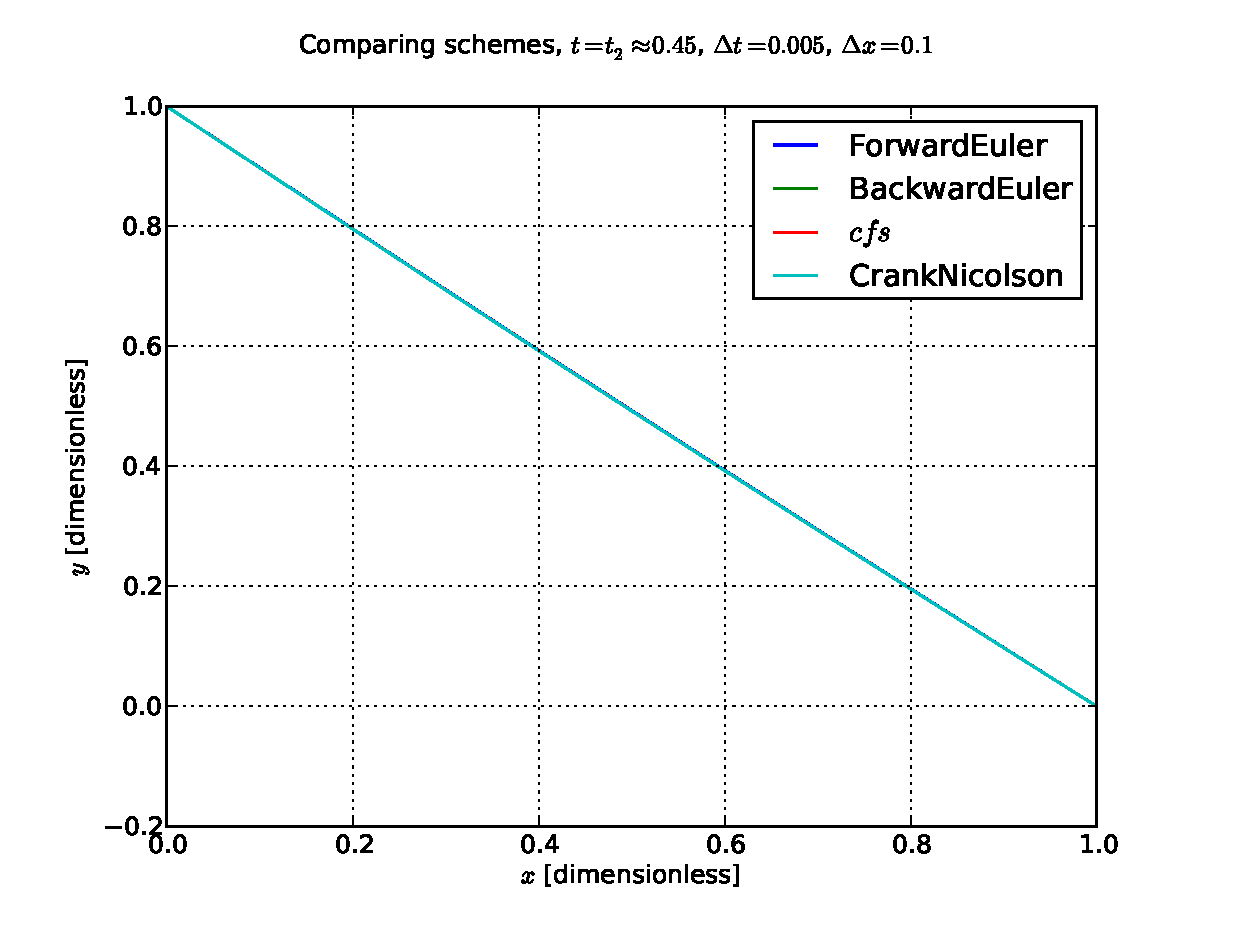
\includegraphics[width=0.9\textwidth]{plots/schemes_case1_t2.eps}
    \caption{A comparison of the different integration schemes for
    test case 1 for the two different time points. Above shows for
    $t_1$ while the lower shows for $t_2$.}
    \label{fig:case1}
\end{figure}

\begin{figure}[htbp]
    \centering
    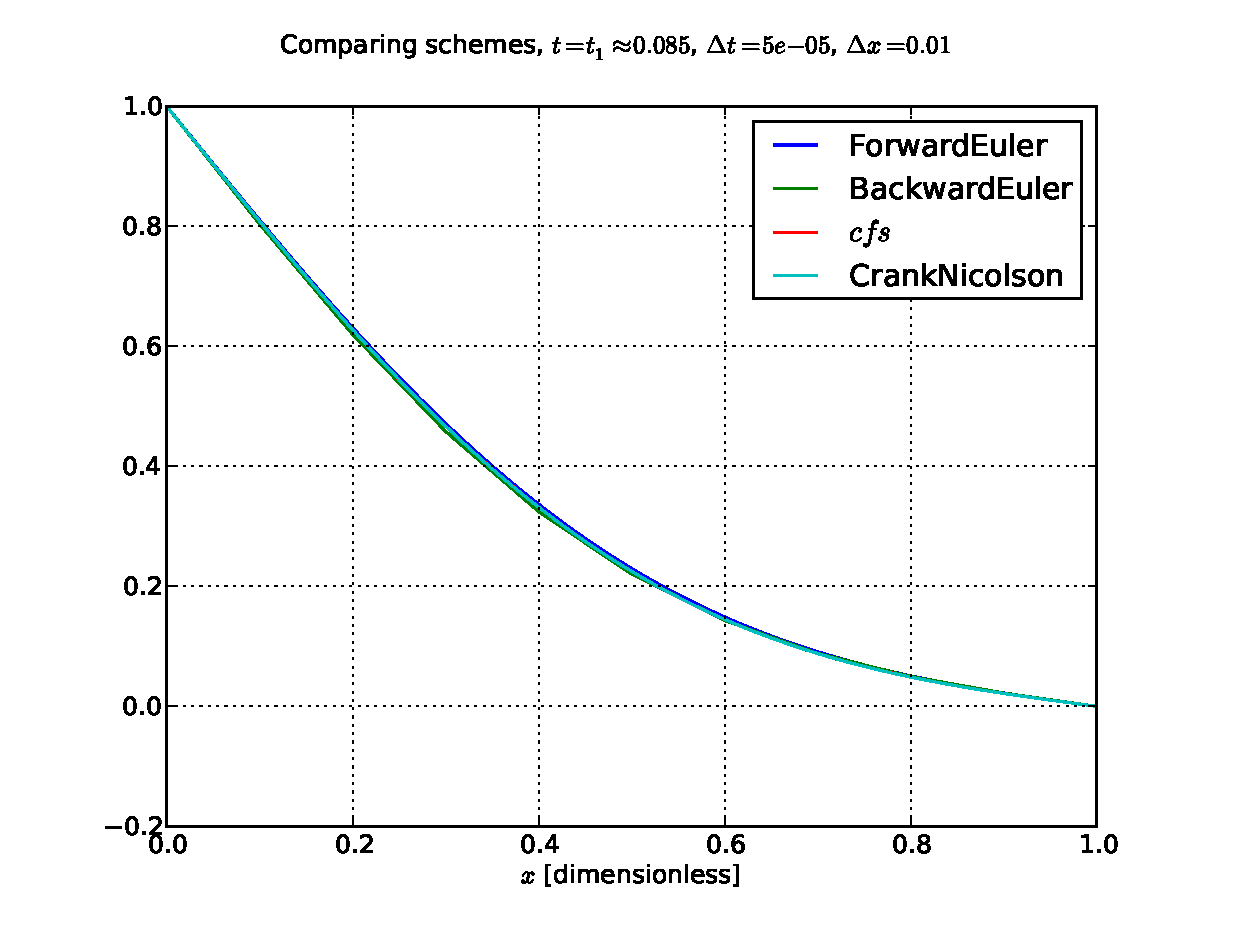
\includegraphics[width=0.9\textwidth]{plots/schemes_case2_t1.eps}
    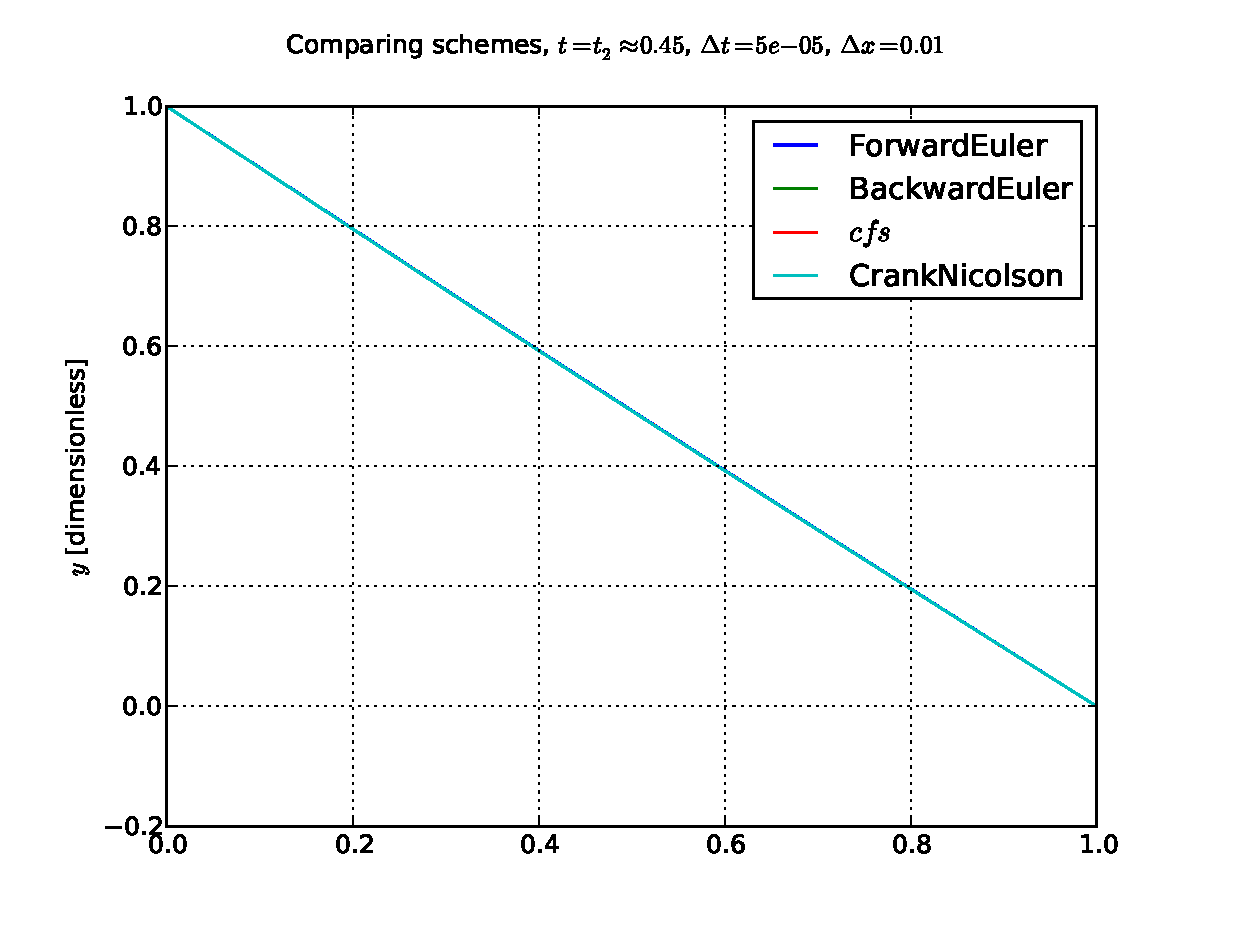
\includegraphics[width=0.9\textwidth]{plots/schemes_case2_t2.eps}
    \caption{A comparison of the different integration schemes for
    test case 2 for the two different time points. Above shows for
    $t_1$ while the lower shows for $t_2$.}
    \label{fig:case2}
\end{figure}

\begin{figure}[htbp]
    \centering
    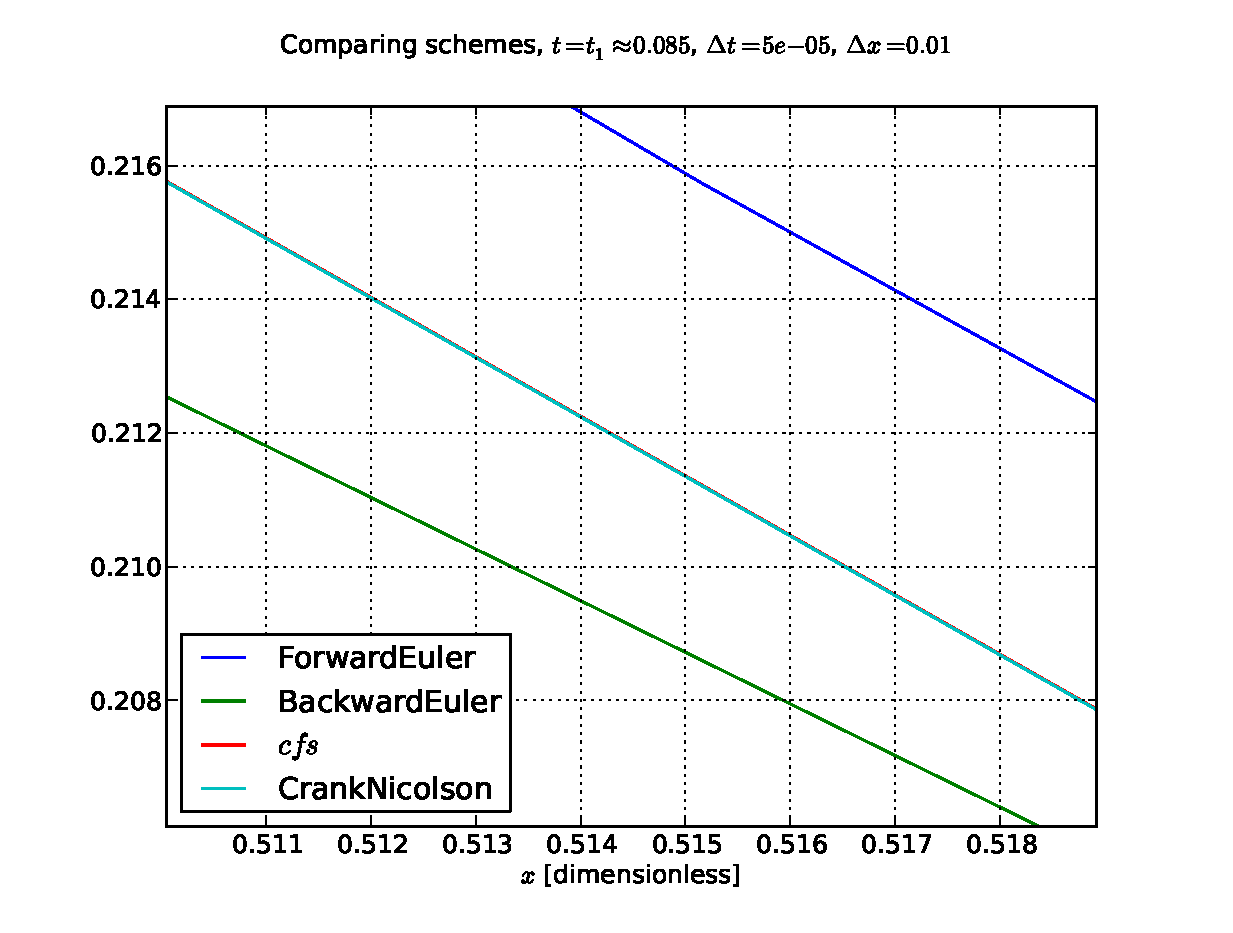
\includegraphics[width=0.9\textwidth]{plots/schemes_case2_t1_zoomed.eps}
    \caption{A comparison of the different integration schemes for
    test case 2 at $t_1$. Notice the ``zoomed'' in scale in order
    to illustrate differences. The closed form solution lies very
    close to the Crank Nicolson solution.}
    \label{fig:zoomed_schemes}
\end{figure}
